%% ------------------------------------------------------------------------- %%
\chapter{Mineração de dados}
\label{cap:mineracao}

A mineração de dados é uma área de pesquisa que almeja a extração de conhecimento útil em uma grande quantidade de dados. Nela concentra-se o foco em buscar padrões e regras previamente desconhecidos usando, entre outras coisas, métodos estatísticos, modelos matemáticos e algoritmos de aprendizado de máquinas \citep{Quboa2013, Kabir2014}. Ela pode ser dividia em três sub-áreas que vão desde a a mineração de dados (\emph{data mining}), a mineração na Web (\emph{web mining}) e a mineração em textos (\emph{text mining}) e varia na manipulação entre dados estruturados e não estruturados \citep{Singh2010}. Enquanto a mineração de mineração de dados lida com dados organizados e estruturados comumente exposto em uma base dados, a mineração de dados em textos, por sua vez, lida com dados não-estruturados. Já a mineração na Web se situa entre os dois extremos combinando técnicas de ambas para aplicar no vasto repositório de documentos da internet \citep{Singh2010, Quboa2013}.

De acordo com o trabalho de \citet{Sleiman2011}, a recuperação da informação útil pode ser facilitada por meio de extratores classificados em dois grupos distintos, os baseados em heurística ou em regras. Além disso, regras de extração de informação podem ser supervisionadas, quando há necessidade de treinamento de um algoritmo, ou não-supervisionadas quando essa necessidade inexiste. As regras comuns de extração de informações e reconhecimento de padrões variam de expressões regulares a gramáticas livres de contexto, regras de primeira ordem, tradutores ou modelos baseados em linguagens especificas como XQuery ou XPath. 

O reconhecimento de padrões pode ser feito de modo manual ou a partir de técnicas supervisionadas de aprendizado de máquinas que variam desde a extração de palavras chaves usando o método tf.idf, conhecido da área de Recuperação de Informação (Information Retrieval), a técnicas que avaliam as estruturas sintáticas do HTML ou a linguagem natural em consideração, até técnicas que extraem a referência para uma estrutura modelo alvo, como uma ontologia \citep{Stumme2006}. Sistemas como o RAPIER \citep{Califf2004} e o BWI \citep{Freitag2000}, por exemplo, fazem essa tarefa a partir de comparação de padrões em volta da informação relevante com a estrutura geral. Já o modelo de \citet{May} se baseia na estrutura sintática dos documentos analisados usando XPath.

A linguagem XPath foi construída de forma a permitir a recuperação a manipulação simples de textos, números ou booleanos em documentos XML \citep{Clark1999} mas também pode ser aplicada a outras documentos com estrutura parecida assim como o HTML. Constituída de uma sintaxe compacta, lembra a notação de caminhos em URLs uma vez que é utilizada tendo em foco a localização de um conteúdo na estrutura hierárquica do arquivo alvo uma vez que o XPath modela um documento XML como uma árvore de nós, incluindo nós de elemento, nós de atributo e nós de texto. Em resumo, ela define uma maneira de calcular um valor de sequência de caracteres para cada tipo de nó. 

Embora existam diferentes técnicas para a mineração de dados em documentos, todas elas técnicas podem ser encapsuladas de maneira tal que uma requisição para um documento, por exemplo, RDF, possa ser reescrita através de um mediador entre cliente e servidor que irá realizar a tradução da requisição da página, extrair a informação relevante e envia-lá ao cliente \citep{Berendt2004, Kushmerick1997}. Isso permite que elas possam ser reaproveitadas dentro de arquiteturas com contextos específicos que não só a mineração de dados.

\section{Mineração de dados para a Web}
\label{sec:mineracao_dados_web}

A mineração Web é um processo de extração de informação ou conhecimento usando diferentes técnicas de mineração como regras de descoberta de associação, agrupamento e classificação aplicadas a fontes de dados expostas na internet \citep{Zhang2011, Quboa2013}. Conforme \citet{Quboa2013} e \citet{Stumme2006} pode ser divida em três categorias (Figura~\ref{fig:hierarquia_mineracao_web}): a mineração de uso na Web, a mineração de conteúdo na Web e a mineração de estrutura na Web. A mineração de uso busca entender o comportamento de um determinado usuário na internet valendo-se dos registros deixados por ele em arquivos de logs como o do navegador Web. Com isso, essa categoria de pesquisa visa criar ou melhorar serviços tornando-os mais personalizados. A mineração de estrutura é uma técnica que tenta reconhecer informações de topologia entre fontes de informações na internet. Ao passo que a mineração de conteúdo atem-se a mineração de informação em textos e imagens a fim de auxiliar uma pessoa a encontrar resultados mais precisos conforme o interesse dela.

\begin{figure}[!ht]
  \centering
  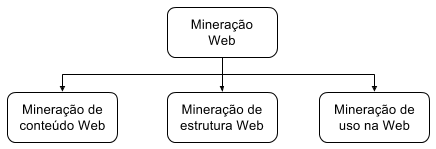
\includegraphics[width=.70\textwidth]{hierarquia_mineracao_web_simplificado} 
  \caption{Categorias da Mineração Web}
\end{figure}
  \label{fig:hierarquia_mineracao_web} 

A mineração de conteúdo é um processo que aproveita a natureza da maioria dos documentos semi-estruturados contidos na Web a partir da exploração de anotações HTML e de suas marcações XML \citep{Stumme2006}. Isso porque essas fontes carregam a informação não somente sobre como uma determinada página deve ser renderizada em um determinado navegador mas também a estrutura lógica delas. Desse modo, ao identificar os padrões de como um determinado texto ocorre em um recurso Web, é possível elaborar processos automatizados para extrair o conteúdo relevante e então mapeá-los para uma nova estrutura que permita um melhor gerenciamento do domínio da informação. Em geral, as técnicas de extração de informação visando à construção da Web semântica dependem muito do reconhecimento da informação em documentos que geralmente é feita a partir da descoberta de padrões \citep{Berendt2004}.

De acordo com \citet{Zhang2011}, a mineração de dados na Web é alcançada por meio de quatro passos conforme ilustra a figura (Figura~\ref{fig:processo_web_mining}): a descoberta de recursos que compreende a a escolha e obtenção de dados de um recurso na Web seja ele um documento eletrônico, um e-mail ou registros de navegação de um usuário. A escolha da informação e o pré-processamento que envolve remover os dados irrelevantes à informação escolhida. A busca automatizada do padrão por meio de ferramentas de mineração como, por exemplo o XPath e a análise do padrão encontrado que envolve a validação por meios automatizados ou a partir da avaliação humana.

\begin{figure}[!ht]
  \centering
  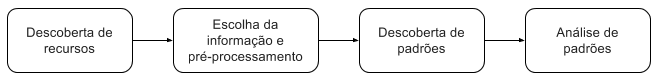
\includegraphics[width=.90\textwidth]{processo_web_mining} 
  \caption{O processo de Web Mining \citep{Zhang2011}}
  \label{fig:processo_web_mining} 
\end{figure}

\section{Mineração de dados para a Web Semântica}
\label{sec:mineracao_web_semantica}

Embora a mineração Web forneça meios para extrair conhecimento relevante na Web, a maioria dos dados espalhados na rede é desestruturada a ponto de tornar complicada a agregação de conteúdos sob uma estrutura comum \citep{Kabir2014}. Nesse contexto, a Web Semântica pode ser combinada com essas técnicas de mineração na internet formando uma área de pesquisa que engloba as área de Mineração de dados e Web Semântica para suprir essa deficiência.

A mineração de dados voltada para a Web semântica (\emph{Semantic Web Mining}) combina o desafio de fazer com que dados sejam compreensíveis para máquinas com o de extrair conhecimento útil escondido nesses documentos de forma automática por meio de técnicas de mineração em dados\cite{Stumme2006}. Esse modo de recuperação de informação é válido tanto em cenários bem estruturados como tabelas em banco de dados, em textos semi-estruturados, ou até naqueles textos sem estrutura alguma, de maneira que podem ser aplicados para ajudar a criar a Web Semântica.



%\section{A linguagem XPath para XML}
%\label{sec:xpath}



%figura do A State-of-the-Art Survey on Semantic Web Mining.png

%\cite{Stumme2006} The first major application area is content mining, i.e., the explicit encoding of semantics for mining theWeb content. The hyperlinks and anchors in a page are part of that page’s text,  and in a semantically marked-up page they are page elements in the same way that text is. So content and structure are strongly intertwined (the two fields are sometimes treated as one [37]). In the SemanticWeb, the distinction between content and structure mining disappears completely, as the content of the page is explicitly turned into the structure of the annotation. However, it should be noted that the distribution of the semantic annotations within a page and across pages may provide additional implicit knowledge.


%\citep{Kabir2014}
%Data mining is a process to extract useful and interesting knowledge from large amount of data. Web Mining aims at discovering insights about the meaning of Web resources and their usage. Given the primarily syntactical nature of the data being mined, the discovery of meaning is impossible based on these data only. Therefore, formalizations of the semantics of Web sites and navigation behavior are becoming more and more common. Semantic Web Mining combines Semantic Web and Web Mining. The nature of most data on the Web is so unstructured that they can only be understood by humans, but the amount of data is so huge that they can only be processed efficiently by machines. The Semantic Web addresses the first part of this challenge by trying to make the data (also) machine understandable, while Web Mining addresses the second part by (semi-)automatically extracting the useful knowledge hidden in these data, and making it available as an aggregation of manageable proportions. Instead of data mining semantic web enables knowledge mining over web.

%\citep{Singh2010}
%Mining the web data is one of the most challenging tasks for the data mining and data management scholars because there are huge heterogeneous,less structured data available on the web and we can easily get overwhelmed with data [2].

%Web Mining visa descobrir insights sobre o significado dos recursos da Web e seu uso. Dada a natureza essencialmente sintática dos dados que estão sendo extraídos, a descoberta do significado é impossível com base nestes dados apenas. Portanto, as formalizações da semântica dos sites e do comportamento da navegação estão se tornando cada vez mais comuns. Semantic Web Mining combina Web Semântica e Web Mining. A natureza da maioria dos dados na Web é tão desestruturada que só pode ser compreendida pelos seres humanos, mas a quantidade de dados é tão grande que só podem ser processados eficientemente por máquinas. A Web Semântica aborda a primeira parte deste desafio tentando tornar a máquina de dados (também) compreensível, enquanto a Web Mining aborda a segunda parte (semi-) extraindo automaticamente o conhecimento útil escondido nesses dados e tornando-o disponível como um Agregação de proporções manejáveis. Em vez de mineração de dados web semântica permite a mineração de conhecimento sobre a web.

%\citep{Sleiman2011}
%The Web is the largest repository of information that has ever existed. This information is presented in a human friendly format using HTML (HyperTextMarkup Language). Unfortu- nately, this format complicates accessing and obtaining this information by automatic processes. Solutions to this problem are the Semantic Web and Web Services, but the lack of such services in the majority of web sites has increased the interest on information extraction.

%\citep{May}
%Appli- cations or users query the agents of the semantic layer via an XML/XPath interface which makes the agent a part of the Semantic Web. The agents then transform the query into another query that actually accesses the underlying sources and return the answer. Each agent contains a knowledge base that semantically describes the concepts of its application domain and con- nects them to the actual data. Thus, an important issue here is to find a modeling and a representation. We use XML as the data model for this level, whereas the actual XML language should be based on a formalism for representing ontological knowledge, e.g., DAML+OIL

%\citep{VanDeursen2008}
%A mapping rule corresponds to an XMLNode element.
%The match attribute indicates the XPath location of the XML node to which the mapping rule will apply. Inside mapping %rules, it is possible to use XPath expressions, as will be discussed further. In case this XPath expression is %relative, the context will be the XML node specified by the XMLNode element.

%1 <XMLtoRDF xmlns:foo="fooNamespace"> <Imports> <Import value="http://foo.com/myOntology.owl"/> </Imports>
%5
%<Vocabularies> <Vocabulary name="voc1">
%<Url>http://foo.com/vocabulary.owl</Url> </Vocabulary> </Vocabularies>
%10
%<XMLNode match="foo:element1"> <!
%</XMLNode> </XMLtoRDF>
%--...-- >
%Listing 1. Basic structure of a mapping document.
%Simple